\documentclass[a4paper,UTF8]{ctexart}

\usepackage{amsmath, amsthm, amssymb, amsfonts, hyperref, mathrsfs}%美国数学学会的包+?
\usepackage{geometry} %控制界面
\usepackage{bookmark}
\usepackage{fancyhdr} % header & footer
\usepackage{appendix} % 附录
\usepackage{tikz} %作图
\usepackage{graphicx} %插入图片的宏包
\usepackage{float} %设置图片浮动位置的宏包
%\usepackage{subfigure} %插入多图时用子图显示的宏包
\usepackage{listings} %引用代码
\usepackage{physics,mathtools} %物理数学工具
\usepackage{comment}
\usepackage{framed}
\usepackage{caption}
\usepackage{subcaption}
\geometry{top=2.5cm,bottom=2.5cm,left=2.5cm,right=2.5cm} % 布局要求
\pagestyle{fancy} % fancy分格
\fancyhf{} % 清除所有页眉页脚
\renewcommand\headrulewidth{0.6pt}
\renewcommand\footrulewidth{0.6pt}
% font
\setCJKmainfont{Noto Serif CJK SC}[BoldFont={Noto Serif CJK SC Bold}, ItalicFont=]
\lhead{何金铭 PB21020660$\mid$座位号:2}
\cfoot{Nd:YAG 激光器自由运转及调Q实验预习报告}
\rhead{\thepage}
\lfoot{2024.4.7}
\rfoot{USTC}
%\bibliographystyle{plain} % 引用样式
\everymath{\displaystyle} % display
%============================================================

\begin{document}

\begin{center}
    \textbf{\Large Nd:YAG 激光器自由运转及调Q实验预习报告}
    \par \text{\large 何金铭 PB21020660}
\end{center}

\section{实验目的}

\begin{enumerate}
    \item 了解固体激光器的结构及工作原理(自由运转和染料调 Q),掌握其调整方法;
    \item 了解固体激光器的主要参数的测试技术;
    \item 观察调 Q 脉冲经过 KTP 晶体实现倍频现象,了解倍频中相位匹配特性。
\end{enumerate}

\section{实验原理}

\subsection{自由振荡}

固体激光器主要由工作物质,泵浦光源和光学谐振腔三大部分组成。其中常用的工作物质为掺钕钇铝石榴石(Nd:YAG)。
且激光器中一个场景的现象是自由振荡,即在没有外界干扰的情况下,激光器自发地产生激光。在自由振荡过程中,激光器的输出光强随时间的变化呈现出一定的规律性。
其特点是具有尖峰结构,即由许多振幅、脉宽和间隔作随机变化的尖峰脉冲组成。每个尖峰的宽度约为 0.1~1 μs,间隔为数微秒,脉冲序列的时间长度大致等于闪光灯泵浦持续的时间。这种现象称为激光器的弛豫振荡。

自由震荡的具体物理过程如下:

\begin{figure}[H]
    \centering
    \begin{minipage}[b]{0.45\textwidth}
        \centering
        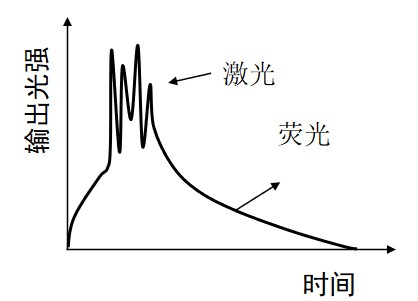
\includegraphics[width=0.9\textwidth]{./fig2.jpg}
        \caption{自由振荡示意图}
    \end{minipage}
    \begin{minipage}[b]{0.45\textwidth}
        \centering
        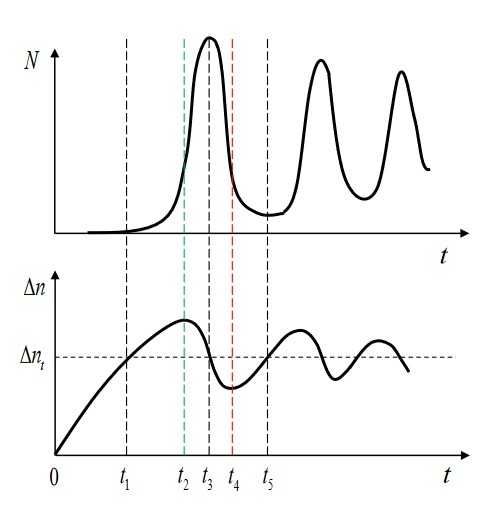
\includegraphics[width=0.9\textwidth]{./fig3.jpg}
        \caption{自由振荡中$N$与$\Delta n$示意图}
    \end{minipage}
\end{figure}

\subsection{染料调Q}

品质因数 $Q$ 是激光器的一个重要参数,它是激光器谐振腔的能量损耗与储存能量之比。调 Q 是指通过改变谐振腔的损耗,使激光器的输出特性发生变化。
其定义为:

\begin{equation}
    Q = 2\pi \nu_0 \frac{W}{\delta W c/nL}
\end{equation}

其中被动调 Q 是利用染料的可饱和吸收特性来完成调 Q 运转的。
其具体利用了染料的可饱和吸收特性。可吸收特性如下图所示:

\begin{figure}[H]
    \centering
    \begin{minipage}[b]{0.9\textwidth}
        \centering
        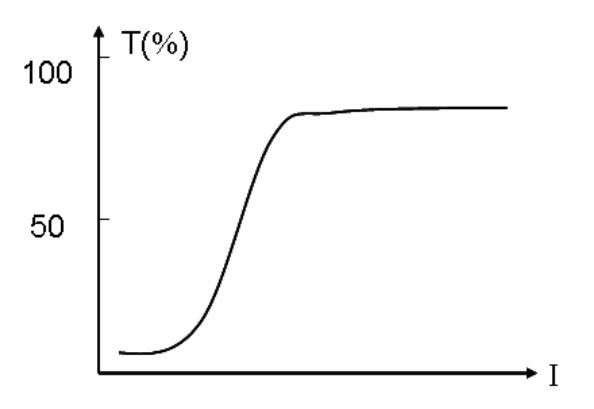
\includegraphics[width=0.9\textwidth]{./fig4.jpg}
        \caption{染料的可饱和吸收特性}
    \end{minipage}
\end{figure}

将具有饱和吸收特性的染料(溶液或固态片)置于谐振腔内。最初,腔内自发荧光很弱,
但染料吸收系数很大,光的透过率很低,腔处于低 Q 值状态,
不能形成激光振荡。随着光泵的继续作用,粒子反转数积累,
腔内荧光逐渐增强,染料吸收系数逐渐减小,透过率逐渐增大。
当光强增为饱和光强$I_s$时,染料吸收达到饱和而变得透明,
此时腔的 Q 值猛增,产生激光振荡,输出调 Q 激光。
因为光泵是脉冲式的,故腔内光场迅速减弱($I\rightarrow 0$),
染料又恢复了吸收特性,接着重复上面的过程。

\subsection{脉冲倍频}

脉冲倍频是指将激光脉冲的频率提高一倍,即将波长减半。倍频的实现需要满足相位匹配条件。

由于晶体中存在色散现象,所以在倍频晶体中的通光方向上,基频光与倍频光所经历的折射率$n_{\omega}$与$n_{2\omega}$是不同的.
当改变晶体中入射光的角度,中间的非常光折射率曲线随之变化.

KTP晶体属于双轴晶体,实验中采用II类相位匹配.经理论计算可得倍频效率为一个Sinc函数的平方函数.
当$\Delta k=0$时效率达到最大值,失配量在$\pi$的整数倍时达到最小值。
\section{实验内容}

\subsection{自由振荡}

\begin{figure}[H]
    \centering
    \begin{minipage}[b]{0.9\textwidth}
        \centering
        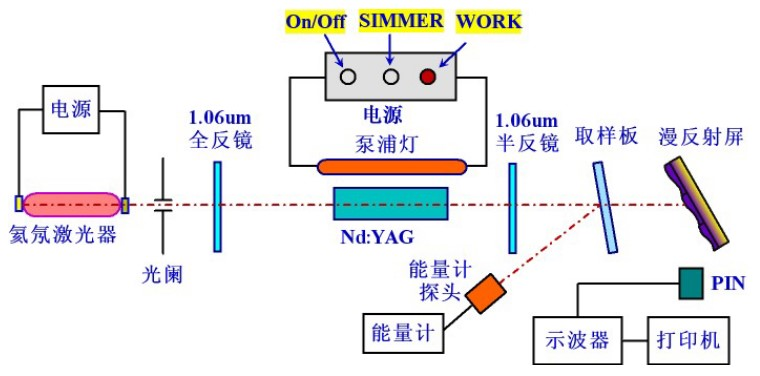
\includegraphics[width=0.9\textwidth]{./fig1.jpg}
        \caption{自由振荡 YAG 激光器光路图}
    \end{minipage}
\end{figure}

本实验的实验目的是用示波器观察激光器的振荡波形,了解激光器的自由振荡特性。

\subsection{染料调Q}

\begin{figure}[H]
    \centering
    \begin{minipage}[b]{0.9\textwidth}
        \centering
        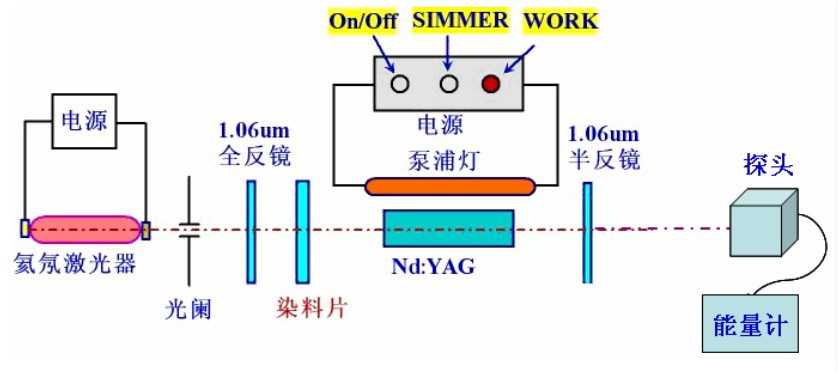
\includegraphics[width=0.9\textwidth]{./fig5.jpg}
        \caption{YAG 激光器调 Q 光路图}
    \end{minipage}
\end{figure}

本实验的目的是用示波器记录激光器的调 Q 脉冲波形,了解调 Q 脉冲的特性。

\subsection{脉冲倍频}

\begin{figure}[H]
    \centering
    \begin{minipage}[b]{0.9\textwidth}
        \centering
        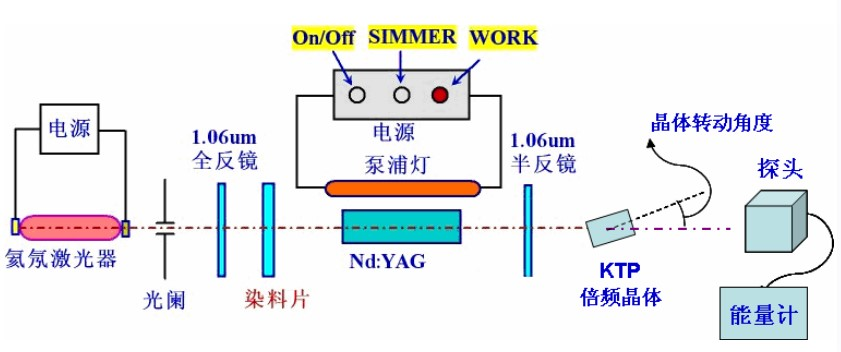
\includegraphics[width=0.9\textwidth]{./fig6.jpg}
        \caption{脉冲倍频实验光路图}
    \end{minipage}
\end{figure}

本实验的目的是转化效率随角度变化的关系图,将获得的拟合曲线和Sinc函数的平方函数进行对比,了解倍频晶体的相位匹配特性。

\end{document}